\section{Accelerating tree construction}\label{sec:accelerating-tree-construction}
Unlike the force calculation part which is easily parallelized, the tree construction step is inherently sequential.
An approach to parallel tree construction outlined in \cite{warren_salmon_1993} involves splitting the set of particles into load-balanced spatial groups which are then used to construct separate trees (one per thread), with the final step being the merge of the created trees.
The merge step is highly involved and beyond the intended scope of this thesis.
For this reason, we propose an alternative approach to accelerating the tree construction which does not involve building the tree in parallel.

Our strategy, based on the ideas put forth in \cite{warren_salmon_1993}, stems from an observation that a potential bottleneck in \autoref{alg:bh-tree-insert} is related to irregular accesses to the nodes of the tree.
Inserting two particles separated by a large spatial distance leads to visiting nodes along two completely different paths in the tree which results in a huge number of cache misses.
A solution to this problem is to sort the list of particles in such a way that subsequent particles on the list (typically) lie close to each other in the physical space.
An ordering with this property can be generated by numbering the particles based on their position along a chosen \textit{space-filling curve}.

A space-filling curve can be thought of as the limit of an infinite sequence of curves that ``fill'' the space without ``holes'' \cite{WeissteinPlaneFilling}.
In the limit, the curve reaches every point of the space, but due to practical constraints, we can only deal with an approximation, i.e. some member of the limiting sequence.
In our implementation, we are working with a \textit{Z-order curve}, also called a \textit{Morton space-filling curve}, so it will in the focus of our discussion.
To make the visualization simpler, assume that the computational domain is two-dimensional and coarsely divided into 16 cells (particles within the same cells are ordered arbitrarily).
Then, the Z-order curve that covers all 16 cells is shown in \autoref{fig:z-order-curve}.
\begin{figure}[htp]
    \centering
    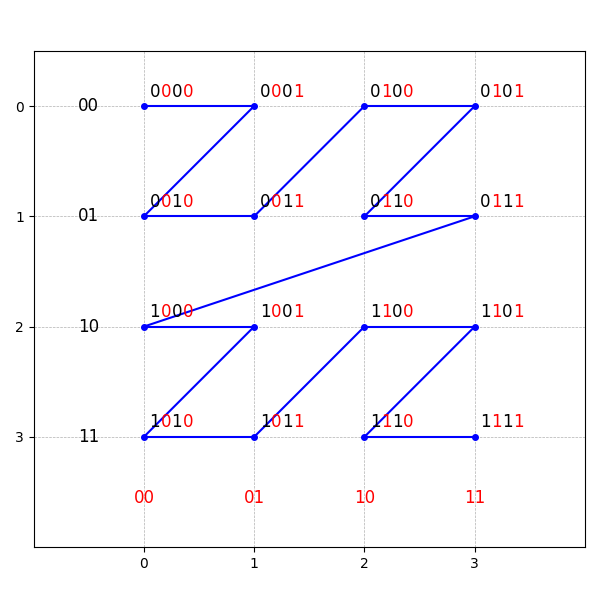
\includegraphics[scale=0.5]{chapters/barnes-hut/img/z-order.png}
    \caption{Z-order curve.}
    \label{fig:z-order-curve}
\end{figure}
The ordering of the points along the curve is obtained by assigning each cell a \textit{Z-value}, whose binary representation is calculated by interleaving the bits of the $x$ and $y$ coordinates.
This is illustrated in \autoref{fig:z-order-curve} by coloring the $x$- and $y$-coordinate bits red and black respectively.

In a standard setting, the coordinates of a particle are given by real numbers and not integers, however.
To establish a mapping between the two, we have to first decide on the intended resolution of the grid.
In our implementation, we use the 32-bit integer type to represent the Z-values, which means that each coordinate should be represented by a 10-bit integer number ($3 \times 10 = 30 \leq 32$).
Thus, the mapping from the real-valued coordinate of a particle to an integer one is given by
\begin{equation*}
    \left\lfloor \frac{(x - \text{low}.x)}{H} \times (2^{10} - 1)\right\rfloor \in [0, 2^{10}),
\end{equation*}
where $\text{low}$ and $H$ define the computational domain as
\begin{equation*}
    \text{domain} = [\text{low}.x, \text{low}.x + H] \times [\text{low}.y, \text{low}.y + H] \times [\text{low}.z, \text{low}.z + H].
\end{equation*}

In our proposed optimization, we make the following changes to the tree construction algorithm (\autoref{alg:bh-tree-insert}):
\begin{enumerate}
    \item The insertion does no longer start at the root of the tree for each particle but at the last inserted to node,
    \item The COM calculation is deferred until the tree construction is finished and carried out using \autoref{eq:bh-com-calculation}.
\end{enumerate}
The second point is a direct consequence of the first one;
if the insertion of a particle does not start at the root but at some other node $n$, deep in the tree, the nodes lying above $n$ will not be updated so their COM and total mass values will be incorrect.
The first point, however, requires more explanation.
Since the particles are z-ordered, subsequent inserts into the tree will result in traversing similar paths.
Because of that, the point of insertion can be found more efficiently by starting the traversal from the last seen node and backtracking up the tree until a valid insertion point is found.
The decision whether to stop backtracking at a given node $n$ is made on the condition that the particle to be inserted is inside a cube represented by $n$.
When the condition is met, the standard insertion procedure takes place starting at $n$.

The asymptotic time complexity of the modified tree construction algorithm is the same as for the standard one.
Sorting the particles requires $O(N\log N)$ operations but inserting a particle into the tree starting at the last-seen node is an $O(1)$ operation.
The last claim may raise objections since some number of backtrack steps are expected on each insert.
To verify it, we measured the average number of backtracks per particle in typical simulations and found that it did not exceed $2.5$ (this can be compared with the number of backtracks required when the particles are not z-ordered; in such a case, we found that in the tested scenarios, on average more than 8 backtracks were typically needed).
Even though the modified algorithm still has the $O(N\log N)$ time complexity, it leads to more predictable memory access patterns which result in noticeably improved performance.
The tree construction time as a function of $N$ is shown in \autoref{fig:z-order-tree-time}.
\begin{figure}[htp]
    \centering
    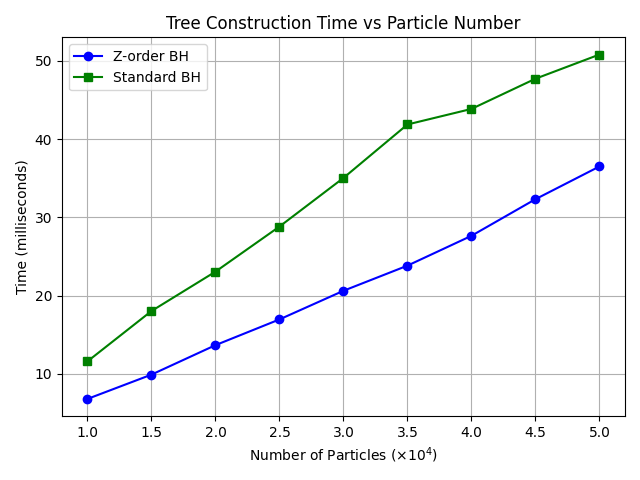
\includegraphics[scale=0.5]{chapters/barnes-hut/img/tree_construction_time.png}
    \caption{Tree construction time averaged over the number iterations of the simulation ($\theta = 1$).}
    \label{fig:z-order-tree-time}
\end{figure}
To generate the graphs shown there, the tree construction time was measured in a spiral galaxy simulation.
As can be seen in the figure, the improved algorithm allows for up to $140\%$ speedup over the standard version.
In our tests, we used the standard library procedure \texttt{std::sort} with the parallel execution policy, which offered a slight speedup over the sequential variant.